% An open problem is the visualization of real-time vehicles data. The problem relies on the fact that most of todays transit APIs will update bus positions about every minute, and therefore some interpolation is needed to animate vehicles on a map. A very rough approach is to update bus position only when there is a new update, but this cause the vehicle to jump from the old position to the new position and makes it difficult to estimate vehicles movement directions; moreover, the vehicle position is out of date until a new update comes. Although a higher frequency for position updates seems desirable it would also increase the battery consumption on your mobile phone querying the requests while also increase the server load that needs to process it. New visualizations should study how to effectively interpolate bus updates, which is not an easy to solve problem. 
  % [see transit_state_of_the_art.pdf P. 8 section 6.4]
  
\subsection{Probleme und Herausforderungen}
\label{sub:probleme_und_herausforderungen}

  Die Visualisierung von Echtzeitdaten bringt einige Schwierigkeiten und Herausforderungen mit sich. Diese werden in diesem Abschnitt gesammelt und beschrieben.

  \subsubsection{Bewältigung der Datenmenge}
  \label{ssub:bewältigung_der_datenmenge}
    An einem Montag den 28.08.2017 zwischen 3.00 und 24.00 Uhr zeigt Abbildung \ref{fig:activeTrips}: Nach einem rapiden Anstieg in der Morgenzeit erreicht die Anzahl an aktiven Trips ihre Maxima um 07.04 mit 779. 

    \begin{figure}[ht]
      \begin{center}
        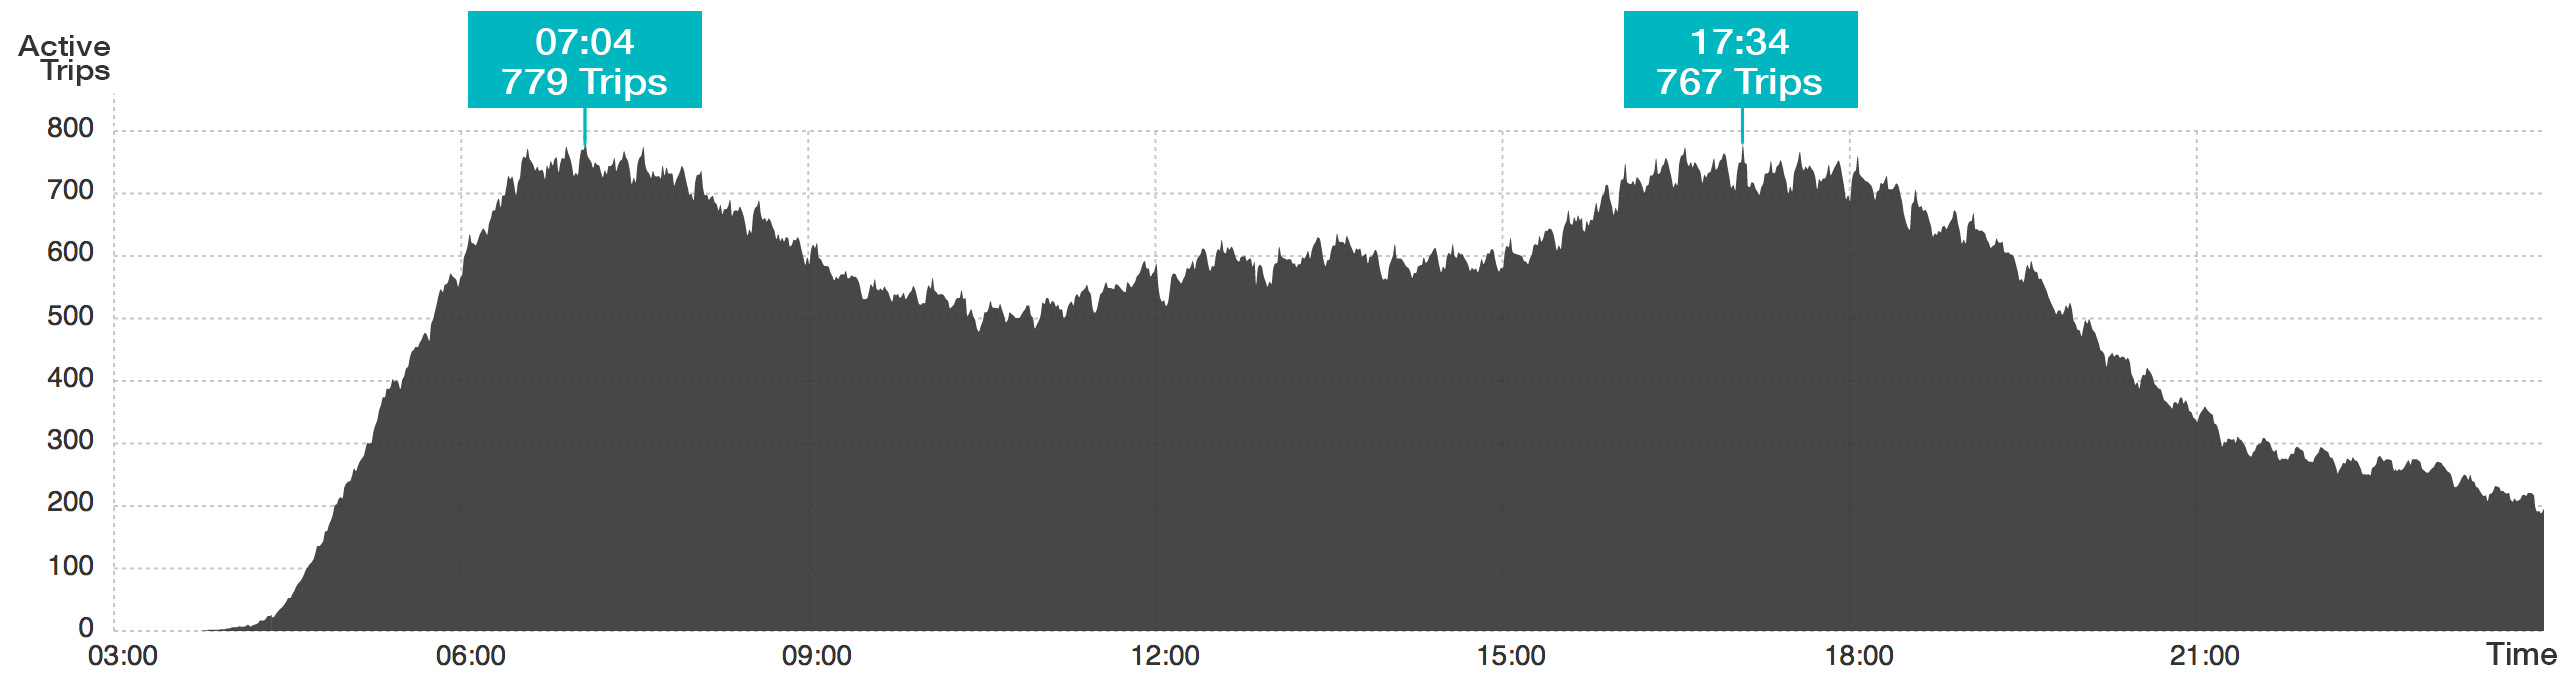
\includegraphics[width=\textwidth]{activeTrips.jpg}
        \caption{Anzahl an aktiven Trips zwischen 3.00 und 24.00 Uhr am 02.08.2017}
        \label{fig:activeTrips}
      \end{center}
    \end{figure}

    Mittags flacht die Anzahl leicht ab, um dann zur Rush Hour am Abend wieder auf 767 gleichzeitig aktive Trips anzusteigen. Anschließend flacht die Anzahl immer weiter ab. Insgesamt wurden an diesem Tag knapp 19650 Trips absolviert. Das Maximum betrug dabei $27 \frac{Trips}{Minute}$ wohingegen das Minimum bei $0 \frac{Trips}{Minute}$ lag. Im Schnitt starten 9 Vehicles pro Minute ihre Fahrt. Für eine interaktive Karte bedeutet dies, dass je nach Tag zwischen 0 und 1000 Trips aktiv sein können. Dies entspricht dann auch der Anzahl an Vehiclen, die sich auf der Karte bewegen und animiert werden müssen. 
  % subsection bewältigung_der_datenmenge (end)